\section{Stochastic Processes}
\label{subsection:stochastic-processes}
There are real-life problems where we consider the evolution of a phenomenon overtime. For example, let $N_0$ be the original number of bacterial cells in the population. The number of bacteria in a population at time $t$ is can be modeled by
\begin{equation}
  \label{example:bacterial-growth}
  N_t = N_0\times 2^t.
\end{equation}

Such model is said to be deterministic. For other problems, such as the evolution of the stock price overtime, deterministic models are not a good selection, since we have to express the risk carefully for every decision on the market. Therefore, randomness should be concerned. In such cases, instead of using such deterministic equation as \ref{example:bacterial-growth}, we allow our equation results in random variables. Hence, we can compute a collection $\{X_t\}_{t\ge0}$ of random variables, which is called a stochastic process.

\subsection{Definitions}

\begin{definition}
  \label{definition:stochastic-process}
  A collection of random variables $\{X_t\}_{t\in I}$ on the same probability space $(\Omega,\F, P)$ is called a stochastic process. For each fixed point $\omega_0\in\Omega$, the map $t\mapsto X(\omega_0, t)$ is called a sample path.
\end{definition}

\begin{remark}
  We can regard a stochastic process as function of two parameters
  $$X:I\times\Omega \to \RR^d.$$
  Hence, sometimes we write $X(t,\omega)$ instead of $X_t(\omega)$. In this case, we assume that $X$ is ($\F\otimes\B(I),\B(\RR^n)$)-measurable.
\end{remark}

\begin{definition}
  Let $\{X_t\}_{t\in I}$ be a stochastic process. If the index set $I$ is countable, then $\{X_t\}_{t\in I}$ is called a discrete-time stochastic process. If $I$ is an interval of $\RR$, then $\{X_t\}_{t\in I}$ is called a continuous-time stochastic process.
\end{definition}

\begin{remark}
  Without loss of generality, if $\{X_t\}_{t\in I}$ is discrete-time, we can choose $I = \NN$, if $\{X_t\}_{t\in I}$ is continuous-time, we will choose $I=\RR$. These selections of the index set are applied for later statements.
\end{remark}

Recall that the $\sigma$-algebra generated by a random variable $X$ is thought of as containing all information about $X$. When a stochastic process evolves overtime, our knowledge about the process increase. For a time $t\in I$, this cumulative information is encapsulated in a $\sigma$-algebra such that all previous random variables $\{X_s\}_{s\in I, s\le t}$ are measurable.

\begin{definition}
  Let $(\Omega, \F, \PP)$ be a probability space. An increasing family $\{\F_t\}_{t\in I}$ of sub-$\sigma$-algebras of $\F$ i.e.
  $$\F_s\subset\F_t \subset \F, \forall t\in I, s\le t$$
  is called a filtration. If
  $$\F_t = \bigcap\limits_{r\ge t} \F_r,$$
  then $\{\F_t\}_{t\in I}$ is said to be right-continuous.

  The tuple $(\Omega, \F, \{\F_t\}_{t\in I}, P)$ is called a filtered probability space.
\end{definition}

\begin{definition}
  Let $(\Omega, \F, \{\F_t\}_{t\in I}, P)$ be a filtered probability space. A stochastic process $\{X_t\}_{t\in I}$ is said to be adapted to the filtration $\{\F_t\}_{t\in I}$ if for any $t\in I$, each random variable $X_s$ where $s\le t$ is $\F_t$ measurable.
\end{definition}

\begin{theorem}
  Let $(\Omega, \F, \PP)$ be a probability space and $\{X_t\}_{t\in I}$ is a stochastic process. Then the family $\{\hat{\F}_t\}_{t\in I}$ of $\sigma$-algebras defined by
  $$\hat{\F}_t = \sigma\left(\left\{\bigcup\limits_{\substack{s\in I \\ s\le t}} \sigma(X_s)\right\}\right)$$
  is a filtration to which $\{X_t\}_{t\in I}$ is adapted. Moreover, the family $\{\hat{\F}_t\}_{t\in I}$ is the smallest adapting filtration i.e. if $\{X_t\}_{t\in I}$ is adapted to another filtration $\{\F_t\}_{t\in I}$, then
  $$\hat{\F}_t \subset \F_t, \forall t\in I.$$
  We called $\{\hat{\F}_t\}_{t\in I}$ the natural filtration \index{natural filtration} of $\{X_t\}_{t\in I}$.
\end{theorem}

We assert the equality of two random variables $X$ and $Y$ in the almost sure sense or in distribution. It is natural to extend this concept of equality to two stochastic processes $\{X_t\}_{t\in I}$ and $\{Y_t\}_{t\in I}$.

\begin{definition}
  Let $(\Omega, \F, \PP)$ be a probability space. Two stochastic processes $\{X_t\}_{t\in I}$ and $\{Y_t\}_{t\in I}$ are said to be indistinguishable \index{indistinguishable} if there exists $A\in\F$ with $P(A)=1$, such that for each
  $$X_t(\omega)= Y_t(\omega), \forall \omega\in A, t\in I.$$
\end{definition}

\begin{definition}
  Let $(\Omega, \F, \PP)$ be a probability space. Let $\{X_t\}_{t\in I}$ and $\{Y_t\}_{t\in I}$ be stochastic processes. We say that $\{X_t\}_{t\in I}$ is a version of $\{Y_t\}_{t\in I}$ if
  $$X_t=Y_t,\,\, a.s \,\,\,\,\forall t\in I.$$
\end{definition}

\begin{remark}
  We can check that ``is a version of'' is an equivalence relation.
\end{remark}

\begin{example}
  \label{example:dis}
  Let $\Omega=I=[0,1]$, $\F=\B(\Omega)$ and $T$ be a random variable distributed uniformly on $\Omega$, $X_t=\mathbf{1}_{t=T}$, then for each $t\in[0,1]$,

  $$P(X_t\ne 0) = P(t=T) = 0.$$

  However, $X_t$ is not indistinguishable from the constant process zero, since there is no subset $A$ of $\Omega$ with $P(A)=1$ such that for each $t\in I$, $X_t(\omega)= 0, \forall \omega\in A.$
\end{example}

For random variables, we adjust the $L^2$ norm in an $L^2$ space to study their convergence in a computationally efficient way. We also create a space $\L^2$ for stochastic processes such that they do not explode. Also, if a sequence $(\{X_n(t)\}_{t\in[0,T]})_{n\in\NN}$ of processes converges to $\{X(t)\}_{t\in[0,T]}$, then it guarantees that for each $t\in[0,T]$,
$$X_n(t) \xrightarrow{n\to\infty} X(t) \text{ in } L^p.$$

\begin{definition}[The $\L^2$ space of stochastic processes]
  Define $\L^2:=\L^2(\Omega, [0,T])$ to be the space of stochastic processes such that for each $\{X_t\}_{t\in [0,T]}\in \L^2$,
  $$\EE\left[\int\limits_0^T X^p_t \d t\right] < \infty.$$
\end{definition}


\begin{theorem}
  The function $\|\cdot\|_{\L^2}:\L^2\to\RR$ defined by
  \begin{equation}
    \|\{X_t\}_{t\in [0,T]}\|_{\L^2} = \left(\EE\left[\int\limits_0^T X^p_t \d t\right]\right)^{1/2}
  \end{equation}
  is a norm on $\L^2$, called the $\L^2$-norm. Moreover, the normed space $(\L^2, \|\cdot\|_{\L^2})$ is Banach.
\end{theorem}

% \begin{proof}

% \end{proof}

\subsection{Wiener Processes}

We introduce a popular stochastic process that appears in the Definition \ref{definition:sde} of a stochastic differential equation.

\begin{definition}
  \label{definition:wiener-process}
  A real-valued stochastic process $\{W_t\}_{t\ge0}$ is called the one-dimensional Wiener process or Brownian motion if
  \begin{enumerate}
    \item $W_0=0$ a.s.
    \item $W(t_2)-W(t_1) \sim \N(0,t-s)$.
    \item Independent increments: for any three times $t_1<t_2<t_3$, the random variables $W(t_2)-W(t_1)$ and $W(t_3)-W(t_2)$ are independent.
    \item The sample path $t\mapsto W(t,\omega)$  is continuous a.s.
  \end{enumerate}
  An $d$-dimensional Wiener process is a vector of $d$ one-dimensional Wiener processes.
\end{definition}

\begin{figure}
  \centering
  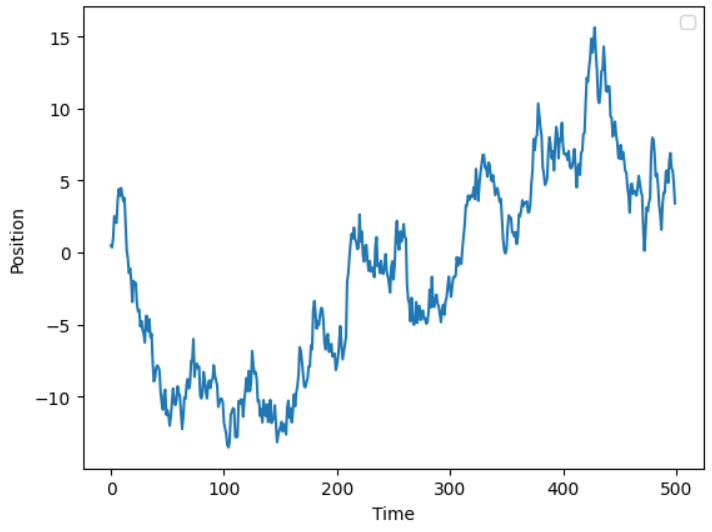
\includegraphics[width=0.5\linewidth]{img/1d-brownian.png}
  \vspace{0.5cm}
  \caption{An illustration of the Wiener process.}
  \label{figure:brownian-motion-illustration}
\end{figure}

\begin{theorem}[Quadratic Variation]
  \label{theorem:quadratic-variation}
  Let $[a, b]$ be an interval in $[0,\infty)$ and partitions
  $$P^n=\{0=t_0^n\le t_1^n\le\ldots\le t_m^n=T\},$$
  with $\left|P^n\right|\to0$ as $n\to\infty$. Then
  \begin{equation}
    \sum\limits_{k=0}^{m_n-1}\left(W\left(t_{k+1}^n\right)-W\left(t_k^n\right)\right)^2\to b-a
  \end{equation}
  as $n\to\infty$.
\end{theorem}

\begin{proof}
  Let $Q_n=\sum\limits_{k=0}^{m_n-1}\left(W\left(t_{k+1}^n\right)-W\left(t_k^n\right)\right)^2$, then
  $$Q_n-(b-a)=\sum\limits_{k=0}^{m_n-1}\left(\left(W\left(t_{k+1}^n\right)-W\left(t_k^n\right)\right)^2-\left(t^n_{k+1}-t^n_k\right)\right).$$

  Hence,
  \begin{align*}
     & \EE[(Q_n-(b-a))^2]                                                                                                                                                                                                                                                                           \\
     & =\sum\limits_{k=0}^{m_n-1}\sum\limits_{j=0}^{m_n-1}\EE  \left[\left(\left(W\left(t_{k+1}^n\right)-W\left(t_k^n\right)\right)^2-\left(t^n_{k+1}-t^n_k\right)\right)\right. \left.\left(\left(W\left(t_{j+1}^n\right)-W\left(t_j^n\right)\right)^2-\left(t^n_{j+1}-t^n_j\right)\right)\right].
  \end{align*}

  If $k\ne j$, due to independent increment, the term becomes the product of two expectations. Since $W(t)-W(s)\sim \N(0,t-s)$ for $t>s\ge 0$, the first expectation is

  $$\EE\left[\left(\left(W\left(t_{k+1}^n\right)-W\left(t_k^n\right)\right)^2-\left(t^n_{k+1}-t^n_k\right)\right)\right]=0.$$

  Therefore, this term vanishes and
  \begin{align*}
    \EE[(Q_n-(b-a))^2]=\sum\limits_{k=0}^{m_n-1}\EE\left[\left(\left(W\left(t_{k+1}^n\right)-W\left(t_k^n\right)\right)^2-\left(t^n_{k+1}-t^n_k\right)\right)^2\right].
  \end{align*}
  Let $Y_k = \dfrac{W\left(t_{k+1}^n\right)-W\left(t_k^n\right)}{\sqrt{t_{k+1}^n-t_k^n}}\sim\N(0,1)$, we have
  \begin{align*}
    \EE\left[\left(\left(W\left(t_{k+1}^n\right)-W\left(t_k^n\right)\right)^2-\left(t^n_{k+1}-t^n_k\right)\right)^2\right] & =\EE\left[(t^n_{k+1}-t^n_k)^2(Y_k^2-1)^2\right]  \\
                                                                                                                           & =(t^n_{k+1}-t^n_k)^2\EE\left[(Y_k^2-1)^2\right].
  \end{align*}
  Let $C=\max\limits_{i=1,\ldots,k}\left\{\EE\left[(Y_k^2-1)^2\right]\right\}$, we have

  $$\EE[(Q_n-(b-a))^2]\le C\sum\limits_{k=0}^{m_n-1}(t^n_{k+1}-t^n_k)^2\to 0 \text{ as } n\to\infty.$$
\end{proof}

Also, every stochastic process is associated with a class of its modifications, whose finite distributions are the same. We say that a stochastic process identifies a \textit{probability law}\index{probability law}. From now on, we denote $P^0$ the probability law of a process starting from time $0$.

\subsection{Markov Processes}

\begin{definition}[Markov Property]
  Let $(\Omega, \F, \PP)$ is a probability space. A stochastic process $\{M_t\}_{t\in[0,T]}$ adapted to a filtration $\{\F_t\}_{t\in[0,T]}$ is a Markov process if
  \begin{equation}
    \EE[M_t|\F_s] = \EE[M_t|M_s],  \forall 0 \le s \le t \le T.
  \end{equation}
  A Markov process is said to be time-homogeneous if $M_t = M_s, a.s.$ for some $t > s$ implies that $M_{t+r} = M_{s+r}, a.s. \forall r\ge0$.
\end{definition}

\begin{definition}[Infinitesimal Generator]
  Let $\{K_t\}$ be a continuous-time semigroup of linear operators on $L^2$. We say that a function $f\in L^2$ belongs to $\mathrm{Dom}(G)$ if the limit
  \begin{equation}
    \lim\limits_{h\downarrow 0}\dfrac{K_hf - K_0f}{h} := Gf
  \end{equation}
  exists in $L^2$. In such cases, $G$ is called the infinitesimal generator of $\{K_t\}$.
\end{definition}

\begin{theorem}[The Derivative of a Function Evolved by a Semi-Group]
  Let $G$ be the generator of a semigroup of linear operators $\{K_t\}$ on $L^2$. For a fixed $f\in\Dom(G)$, set $u(x,t) := (K_tf)(x)$. Then $\partial_t u$ exists for all $t$, and is equal to $Gu$.
\end{theorem}
% \begin{proof}

% \end{proof}

\begin{definition}[Self-space Markov Kernel]
  Let $(\Omega, \F)$ be a measurable space. A function $\kappa: \Omega\times\F\to[0,1]$ is called a (self-space) Markov kernel on $(\Omega, \F)$  if
  \begin{enumerate}[label=(\roman*), ref=(\roman*)]
    \item For any $F\in\F$, the function $\kappa(\cdot, F): \Omega \to [0,1]$ is $\F$-measurable.
    \item For any $\omega\in\Omega$, the function $\kappa(\omega, \cdot): \F\to [0,1]$ is a probability measure on $(\Omega, \F)$.
  \end{enumerate}
\end{definition}

\begin{definition}
  Let $(\Omega, \F)$ be a measurable space. Let $\kappa_1$ and $\kappa_2$ be Markov kernels. The product $\kappa_1\kappa_2 : \Omega \to \F$ is a Markov kernel, defined as
  \begin{equation}
    (\kappa_1\kappa_2)(x,F) = \int_{y\in\Omega}\kappa_2(y,F)\d\kappa_1(x,y).
  \end{equation}
\end{definition}

\begin{definition}[Transition Kernel]
  Let $(\Omega, \F)$ be a measurable space. For every $0\le s\le t\le T$, let $\kappa_{s,t}$ be a Markov kernel on $(\Omega, \F)$. The family $\{\kappa_{s,t}\}$ is called a semigroup of transition kernels if
  \begin{enumerate}[label=(\roman*), ref=(\roman*)]
    \item For any  $t$, $\kappa_{t,t}(x,B) = \delta_{B}(x)$.
    \item For any $0\le r\le s\le t\le T$, $\kappa_{r,t} = \kappa_{r,s}\kappa_{s,t}$.
  \end{enumerate}
\end{definition}

\begin{definition}
  Let $(\Omega, \F)$ be a measurable space and $\{\kappa_{s,t}\}$ is a semigroup of transition kernels. We define $\{K_{s,t}\}$ the semigroup of transition operators on $B(\RR^d,\RR)$ as
  \begin{equation}
    (K_{s,t}f)(x) = \int\limits_{y\in\Omega}f(y)\d \kappa(x,y) := \kappa_{s,t}(f(x)), \forall x\in\RR^d.
  \end{equation}
\end{definition}

\begin{theorem}[Transition Operator Semigroups and Markov Processes]
  Let $X$ be a Markov process with transition kernels $\{\mu_{s,t}\}$, and let $\{K_{s,t}\}$ be the corresponding semigroup of transition operators. Then for any $f \in B(\RR^d, \RR)$, we have
  \begin{equation}
    \label{equation:transition-operator-semigroups-and-markov-process}
    \EE[X_t | \F_s] = (K_{s,t}f)(X_s).
  \end{equation}
  Conversely, let $X$ be any stochastic process, and let $K_{s,t}$ be a semigroup of transition operators such that Equation \ref{equation:transition-operator-semigroups-and-markov-process} is valid (a.s.). Then $X$ is a Markov process.
\end{theorem}
\begin{proof}
  We have
  \begin{align*}
    (K_{s,t}f)(X_s)
     & = \int\limits_{y\in\Omega}f(y)\d \kappa_{s,t}(x,y) \\
     & = \E[f(X_t) | \sigma(X_s)]                         \\
     & = \EE[X_t | \F_s].
  \end{align*}
\end{proof}

\begin{definition}[Martingale Problem]
  Let $G$ be a generator on $\D\subset\C_b(\RR^d, \RR)$. A $d$-dimensional stochastic process $X:=\{X_t\}$ is a solution to the martingale problem for $G$, $\D$, if for any $f\in \D$,
  \begin{equation}
    f(X_t) - \int\limits_0^t Gf(X_s)\d s
  \end{equation}
  is a martingale with respect to ${\F^X_t}$, the natural filtration of X.
\end{definition}

\begin{lemma}
  A stochastic process $X:=\{X_t\}$ is a solution to the martingale problem if and only if
  \begin{equation}
    \EE\left[f(X_t)|\F^X_s\right] - \EE\left[\left.\int\limits_{s}^t Gf(X_r)\d r \right| \F^X_s\right] = f(X_s), \forall 0\le s\le t\le T.
  \end{equation}
\end{lemma}
% \begin{proof}

% \end{proof}

\begin{theorem}
  Let $X$ be a homogeneous Markov process with generator $G$ and cadlag sample paths. Then X solves the martingale problem for $G$, $\C_b(\RR^d, \RR)\cap \mathrm{Dom}(G)$.
\end{theorem}

\begin{definition}
  Let $(\Omega, \F)$ is a probability space. A function $\kappa: \F \times \RR \to [0,1]$ is called a probability kernel.
\end{definition}

\begin{definition}
  Let $\kappa_1$ and $\kappa_2$ be probability kernels. The product of $\kappa_1$ and $\kappa_2$ is defined as
  \begin{equation}
    (\kappa_1\kappa_2)(x, D) = \int\kappa_1(x, D)\d\kappa(x, y).
  \end{equation}
\end{definition}

\begin{definition}
  Let $\D$ be the set of all distributions on $\RR^d$. For every $s,t$, a probability kernel $\kappa_{s,t} : \D \times \D \to [0,1]$ is called a transition kernel if
  \begin{enumerate}[label = (\roman*)]
    \item For all $t\in[0,T]$ and $D\in\D$, $\kappa_{t,t}(D, ) = \mathbf{1}_{D}(\cdot)$.
    \item For any $r\le s\le t$, $\kappa_{r,t}=  \kappa_{r,s}\kappa_{s,t}$.
  \end{enumerate}
  We usually call $\{\kappa_{s,t}\}$ a transition semigroup.
\end{definition}

Each Markov process is associated with a transition semigroup. Conversely, given a transition semigroup, there exists a corresponding Markov process.

